\documentclass[addpoints]{exam}
\usepackage[utf8]{inputenc}
\usepackage{multicol}
\usepackage{graphicx}
\usepackage{amsmath}
\usepackage[a4paper,top=15mm, bottom=15mm, left=15mm, right=15mm]{geometry}
 
\begin{document}
 
 \begin{center}
\fbox{\fbox{\parbox{5.5in}{\centering Istituti Card. C. Baronio - Vicenza \\ Anno scolastico 2018/2019 \\ Compito di Informatica \\ Schema logico ed SQL}}}
\end{center}
 
\vspace{5mm}
 
\makebox[\textwidth]{Nome e Cognome:\enspace\hrulefill Data e Classe:\enspace\hrulefill}
 
\vspace{5mm}
 
 
\begin{figure}[h!]
	\centering
	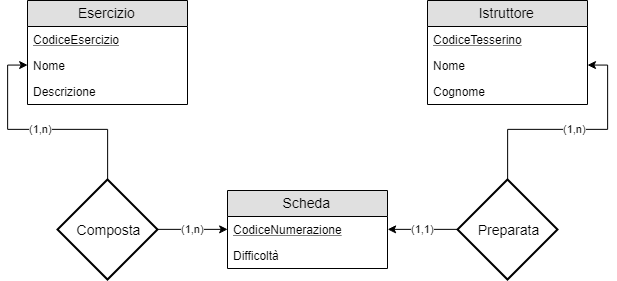
\includegraphics[scale=0.5]{Palestra.png}
\end{figure}

\begin{questions}
	\question Osserva il diagramma soprastante e:
	\begin{parts}
		\part[3] A partire dal diagramma ER fornito, fornisci il corrispettivo schema logico
		\part[2] Crea le tabelle dello schema logico;
		\part[1] Inserisci nella tabella ISTRUTTORE i valori "T001", "Mario", "Rossi" e nella tabella ESERCIZIO i valori "E005", "Squat", "Piegarsi con le ginocchia";
		\part[1] Visualizza tutte le schede con difficoltà "Difficile"
		\part[1] Visualizza il nome e cognome degli istruttori che hanno proposto una scheda con difficoltà "Facile"
		\part[2] Visualizza le difficoltà delle schede create da "Luca" che contengono gli esercizi con nome "addominali" 
	\end{parts}
	\question Osserva il diagramma sottostante e:
	\begin{parts}
		\part[3] A partire dal diagramma ER fornito, crea il corrispettivo schema logico
		\part[2] Crea le tabelle dello schema logico;
		\part[1] Inserisci nella tabella Cliente i valori "C005", "Rossi", "Mario" e nella tabella Oggetto i valori "B548", "Casa", "Bene immobile", "300000"
		\part[1] Visualizza tutte le polizze create il giorno 24/12/2018
		\part[1] Visualizza il nome di tutte le polizze create da "Luca Ferrari"
		\part[2] Visualizza il valore di tutti gli oggetti assicurati dal signor Ferrari
	\end{parts}
\end{questions}

\begin{figure}[h!]
	\centering
	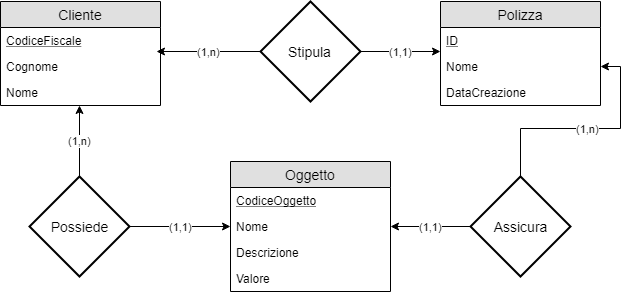
\includegraphics[scale=0.5]{PolizzaAssicurativa.png}
\end{figure}

\begin{center}
	\gradetable[h][questions]
\end{center}

\end{document}